\documentclass[../main.tex]{subfiles}
% DOCUMENT

\begin{document}

\chapter{Bài toán MDP}\label{giux1ea3i-buxe0i-touxe1n-mdp}

Khoá luận sẽ chỉ tập trung vào trường hợp mạng có thuộc tính
\emph{FIFO ngặt}: với mọi cung trong mạng, không thể đi đến cuối một cung sớm hơn bằng cách khởi hành ở thời điểm sau đó.

Trước khi đi vào các chi tiết về cách giải và ví dụ minh họa, cần làm rõ hai yếu tố sau:
\begin{itemize}
  \item \textbf{Đầu vào:} Một mạng thời gian \(D = (N, A)\); khung thời gian \([0, T]\); hàm vận tốc \(c_{i,j}(t)\) tuyến tính từng khúc dưới dạng danh sách cạnh và tập hợp các giá trị tại từng BP. Các BP ở đây đều có thời gian là số nguyên.
  \item \textbf{Đầu ra:} Đường đi có thời gian di chuyển tối thiểu từ đỉnh nguồn đến đỉnh đích. Ngoài ra còn có các thông tin khác đề cập ở phần \autoref{cuxe1c-thux1eed-nghiux1ec7m}.
\end{itemize}

\section{Ví dụ}\label{vuxed-dux1ee5}

Xét mạng ở \autoref{fig:2} với các hàm vận tốc được biểu diễn ở \autoref{fig:4}. 
Khung thời gian là \([0, 5]\). Hầu hết các cung có số BP là số
nguyên. Ngoại lệ là cung \((3, 4)\) chỉ có BP tại \(0, 1, 2\) và
\(5\). \autoref{appendix-arc4} cung cấp chi tiết về các hàm vận tốc và các hàm \emph{đảo chiều} của ví dụ này.



\begin{figure}[h]
\centering
\begin{minipage}{0.45\textwidth}
  \centering
  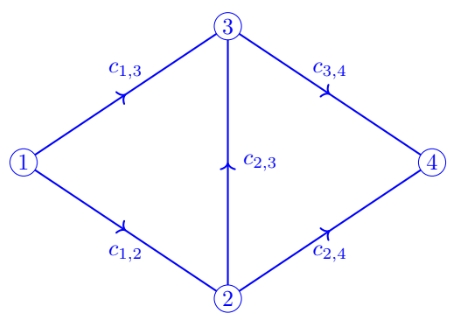
\includegraphics{edited-images/Figure2.jpg}
  \caption{Mạng \(D\)}
  \label{fig:2}
\end{minipage}
\begin{minipage}{0.49\textwidth}
  \centering

      \captionof{table}{Bảng Thời gian di chuyển với mỗi BP}
      \label{table:1}
      \resizebox{0.8\linewidth}{!}{%
        \begin{tabular}{|c||ccccc|}
        \toprule
        \multirow{2}{*}{BP} & \multicolumn{5}{c|}{Cung di chuyển}                                                                                       \\ \cmidrule{2-6} 
                            & \multicolumn{1}{c|}{(1,2)} & \multicolumn{1}{c|}{(1,3)} & \multicolumn{1}{c|}{(2,3)} & \multicolumn{1}{c|}{(2,4)} & (3,4) \\ \midrule
        0                   & \multicolumn{1}{c|}{1.34}  & \multicolumn{1}{c|}{2.85}  & \multicolumn{1}{c|}{1.99}  & \multicolumn{1}{c|}{1.29}  & 0.61  \\ \midrule
        1                   & \multicolumn{1}{c|}{0.66}  & \multicolumn{1}{c|}{2.95}  & \multicolumn{1}{c|}{1.82}  & \multicolumn{1}{c|}{1.02}  & 0.73  \\ \midrule
        2                   & \multicolumn{1}{c|}{0.14}  & \multicolumn{1}{c|}{3.00}  & \multicolumn{1}{c|}{1.51}  & \multicolumn{1}{c|}{1.63}  & 0.83  \\ \midrule
        3                   & \multicolumn{1}{c|}{0.01}  & \multicolumn{1}{c|}{2.98}  & \multicolumn{1}{c|}{1.10}  & \multicolumn{1}{c|}{2.57}  & ---     \\ \midrule
        4                   & \multicolumn{1}{c|}{0.35}  & \multicolumn{1}{c|}{2.90}  & \multicolumn{1}{c|}{0.67}  & \multicolumn{1}{c|}{3.00}  & ---     \\ \midrule
        5                   & \multicolumn{1}{c|}{1.00}  & \multicolumn{1}{c|}{2.76}  & \multicolumn{1}{c|}{0.30}  & \multicolumn{1}{c|}{2.54}  & 1.00  \\ \bottomrule
        \end{tabular}
      }
\end{minipage}

\end{figure}




\begin{figure}[H]
\centering
% 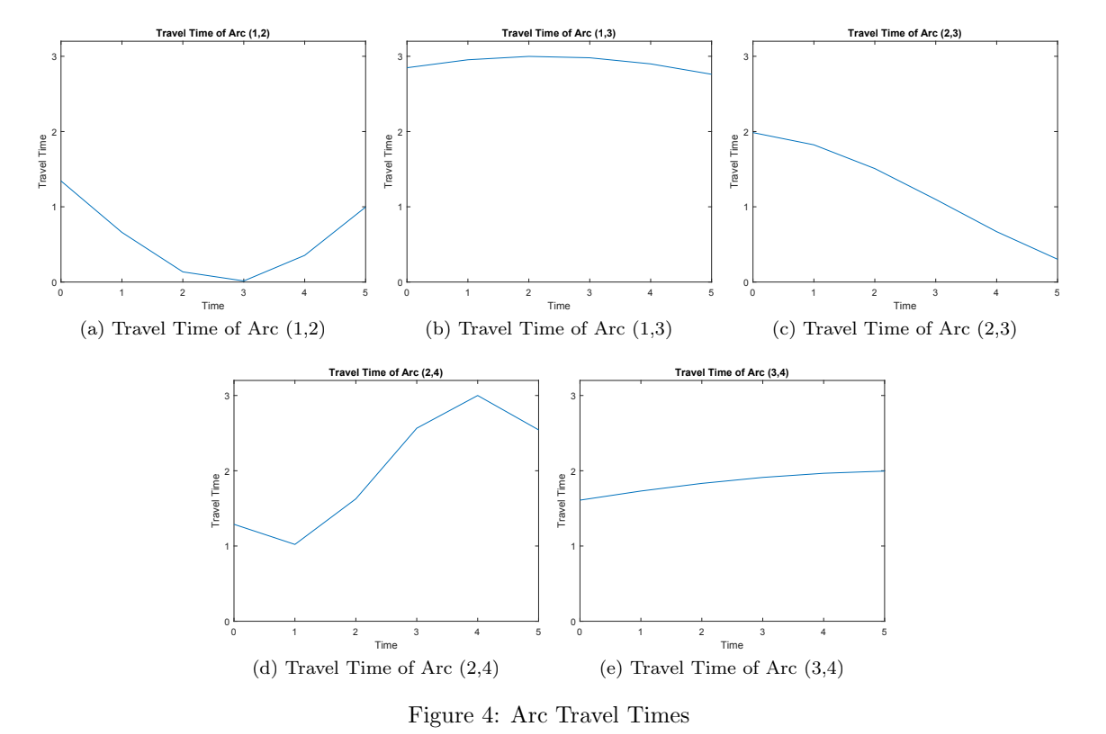
\includegraphics{images/Figure4.png}
\subcaptionbox{Cung \((1,2)\)\label{fig:4a}}{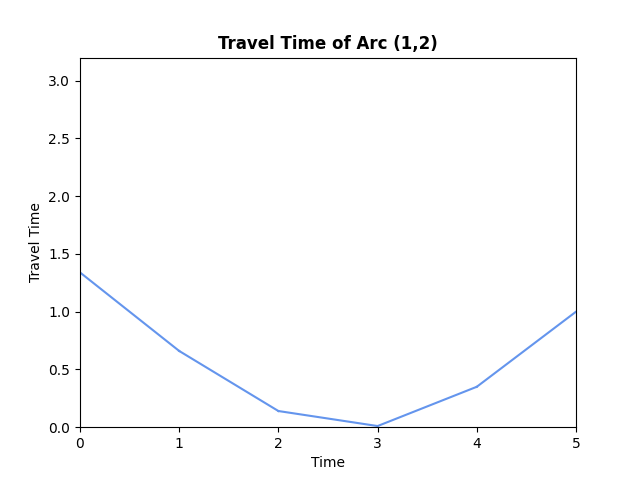
\includegraphics[width=.32\textwidth]{plot/Arc (1,2).png}}
\subcaptionbox{Cung \((1,3)\)\label{fig:4b}}{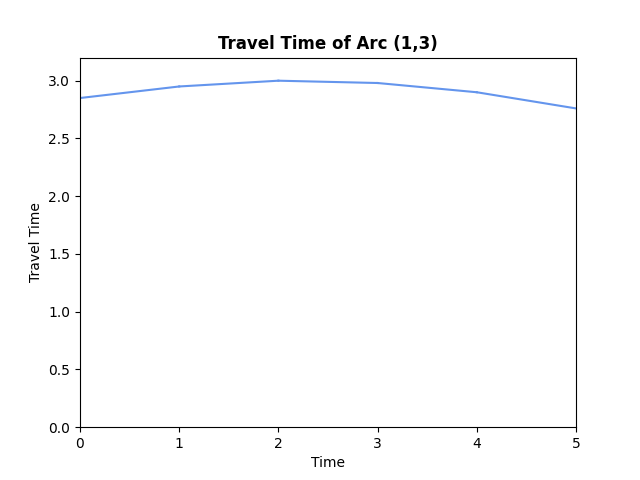
\includegraphics[width=.32\textwidth]{plot/Arc (1,3).png}}
\subcaptionbox{Cung \((2,3)\)\label{fig:4c}}{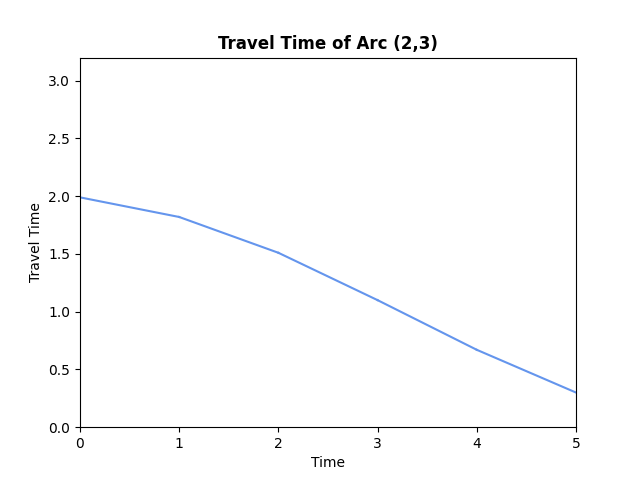
\includegraphics[width=.32\textwidth]{plot/Arc (2,3).png}}

\subcaptionbox{Cung \((2,4)\)\label{fig:4d}}{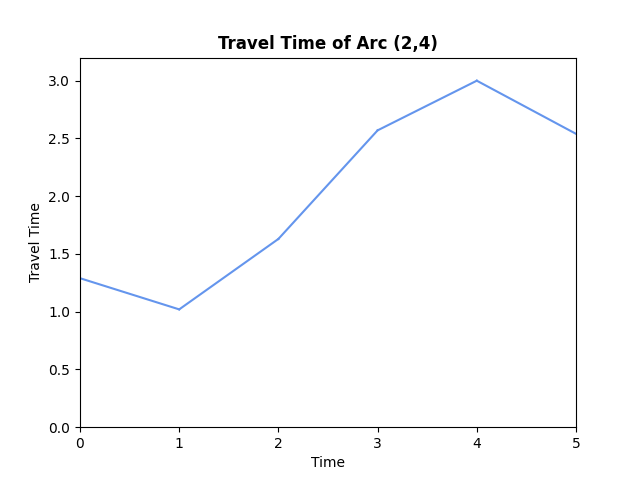
\includegraphics[width=.32\textwidth]{plot/Arc (2,4).png}}
\subcaptionbox{Cung \((3,4)\)\label{fig:4e}}{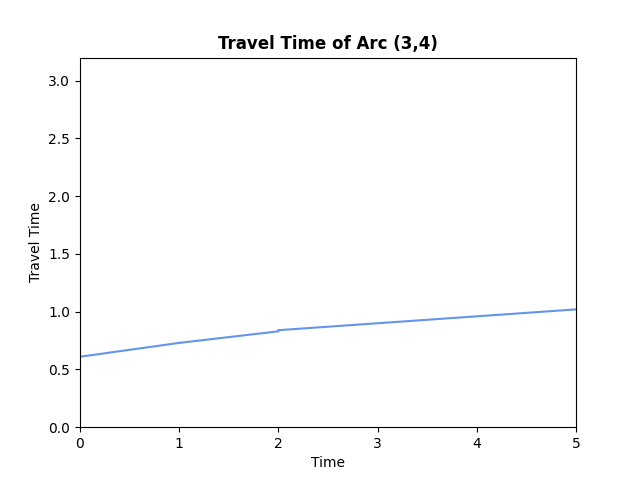
\includegraphics[width=.32\textwidth]{plot/Arc (3,4).png}}

\caption{Biểu đồ đường cho Hàm vận tốc.}
\label{fig:4}

\end{figure}


\section{Công thức chi tiết}\label{cong-thuc1}

Cho thời điểm \(t\) bất kỳ thuộc khoảng \([0, T]\) biểu diễn thời gian
đi đến đỉnh \(n\), ta có thể xây dựng BSPT tương ứng. BSPT là một Mạng
thời gian-không gian (\textbf{TEN}) được kí hiệu là \(B^t\), luôn có gốc là
\((n, t)\). Cây này được định nghĩa bởi tập hợp các nút\footnote{để phân
  biệt mạng với đồ thị, sử dụng từ \emph{nút} thay cho \emph{đỉnh}.} \((i, t_i)\)
với \(i \in N\) và \(t_i \in (-\infty, T]\), tập hợp các cung\footnote{để
  phân biệt mạng với đồ thị, sử dụng từ \emph{cung} thay cho \emph{cạnh}.}
\(((i, t_i), (j, t_j))\) thỏa mãn các điều kiện sau: 

\begin{itemize}
\tightlist
\item
  Với mỗi \(i\in N\), chỉ tồn tại \(t_i\) là thời gian khởi hành muộn
  nhất để đi từ \(i\) đến \(n\). Lúc này \((i, t_i)\in B^t\),
\item
  Cung \((i, j) \in A\),
\item
  \(t_i + c_{i, j}(t_i) = t_j\), và
\item
  \textbf{Chỉ có một đường đi duy nhất}~từ \(i\) đến \(n\) trong
  \(B^t\). Đường đi này được xác định bởi việc thực hiện \emph{TDSP} bắt đầu từ \(i\) tại thời gian \(t_i\) và kết thúc
  ở \(n\).
\end{itemize}

\textbf{BSPT} được tạo từ nghiệm của TDSP (là một đường đi) bằng cách áp dụng thuật toán tìm đường 
đi ngắn nhất từ một đỉnh (Dijkstra)
với một vài điều chỉnh đơn giản liên quan đến chọn các BP thay vì trọng số cố định như thông thường. 
BSPT cho đỉnh \(4\) tại thời gian
\(t=2.57\) được biểu diễn ở \autoref{fig:5b}. Mạng TEN này bao gồm các nút
\(\{(1, 0.00), (2, 1.34), (3, 1.76), (4, 2.57)\}\)\footnote{thời gian
  làm tròn thời gian đến 2 chữ số thập phân} và các cung
\((1, 2), (2, 4), (3, 4)\) được xác định bởi các nút theo thời gian.

\begin{figure}[H]

\centering
% 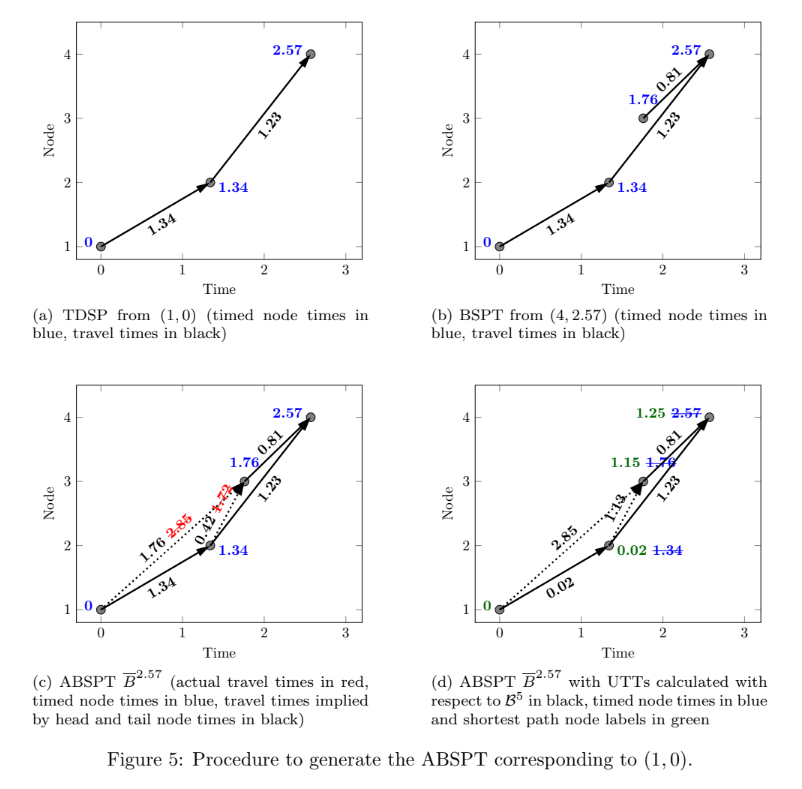
\includegraphics{images/Figure5.png}
\subcaptionbox{TDSP từ nút \((1,0)\)\label{fig:5a}}{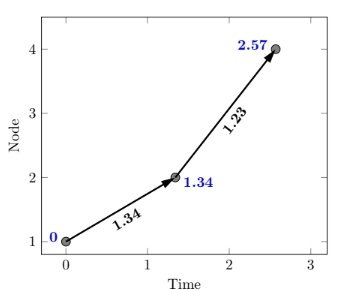
\includegraphics[width=.4\textwidth]{edited-images/Figure5a.jpg}}
\subcaptionbox{BSPT có gốc \((4, 2.57)\)\label{fig:5b}}{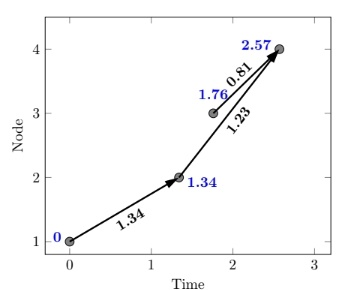
\includegraphics[width=.4\textwidth]{edited-images/Figure5b.jpg}}

\subcaptionbox{ABSPT \(\overline{\mathcal{B}}^{2.57}\)\label{fig:5c}}{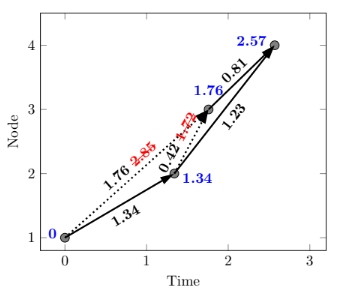
\includegraphics[width=.4\textwidth]{edited-images/Figure5c.jpg}}
\subcaptionbox{ABSPT \(\overline{\mathcal{B}}^{2.57}\) với các UTT khi ghép với \(\overline{\mathcal{B}}^{5}\)\label{fig:5d}}{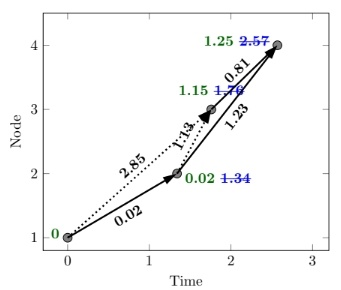
\includegraphics[width=.4\textwidth]{edited-images/Figure5d.jpg}}
\caption{Quy trình tạo ABSPT ứng với
đỉnh xuất phát (1,0)}
\label{fig:5}
\end{figure}

\newpage
Giải thích \autoref{fig:5}: 
\begin{itemize}
  \item \autoref{fig:5a}: đường đi TDSP từ đỉnh \((1, 0)\) đến \(n\) với thời gian là \(2.57\). 
  Các nút thời gian màu xanh, giá trị hàm vận tốc màu đen.
  \item \autoref{fig:5b}: BSPT tương ứng với đỉnh \((4, 2.57)\).
  \item \autoref{fig:5c}: ABSPT \(\overline{\mathcal{B}}^{2.57}\) tương ứng với đỉnh \((4, 2.57)\). 
  Thời gian di chuyển thực tế có màu đỏ.
  \item \autoref{fig:5d}: ABSPT \(\overline{\mathcal{B}}^{2.57}\) với các UTT khi ghép với \(\overline{\mathcal{B}}^5\) (có màu đen),
  đường đi tối thiểu có màu xanh lá.
\end{itemize}

Một vài lưu ý khi xây dựng BSPT \(B^t\) như sau:

\begin{easylist}[itemize]

  @ Tại một thời điểm \(t \in [0, T]\) \textbf{bất kỳ,}~có thể tồn tại một
  số đỉnh \(i\) không thể đi đến đỉnh \(n\)~bất kể với thời gian nào
  \(> 0\).
  @ \textbf{Trường hợp đơn giản:}\\
  Nếu đỉnh đang xét \(i\) ở~thời gian
  \(t = T\), ta có thể loại bỏ nút \(i\) khỏi mạng ngay từ bước xử lý
  trước.
  @ \textbf{Trường hợp phức tạp:}\\
  Để đơn giản hóa cho bước tiếp theo, ta
  giả sử rằng \emph{BSPT} chứa một nút cho mọi đỉnh \(i \in N\). Để thực
  hiện điều này, hàm vận tốc \(c_{i,j}(t)\) được mở rộng
  sang \(t < 0\) (âm): Với mọi cung \((i, j)\) trong mạng \(A\) và mọi
  thời điểm \(t < 0\), ta gán giá trị của \(c_{i,j}(t) = c_{i,j}(0)\).
  Do đó, các nút \((i, t_i)\) với \(t_i<0\) cũng có thể được thêm vào
  mạng \(B^t\).
\end{easylist}

Thuật toán DDD được xây dựng dựa trên những đặc điểm sau của các BSPT: 
\begin{itemize}
  \tightlist
  \item
    \textbf{Tính chất FIFO:}\\ 
    Nếu hai nút \((i, s)\) trong \(B^t\) và
    \((i, s')\) trong \(B^{t'}\) với \(t' > t\) thì \(s' > s\) (điều này
    có nghĩa là nếu một nút đến muộn hơn trong \(B^t\), nó cũng sẽ đến
    càng muộn hơn trong \(B^{t'}\)).
  \item
    \textbf{Đường đi theo thời gian tối thiểu:} \\
    Bất kỳ đường đi có thời
    gian tối thiểu nào từ đỉnh \(1\) đến \(n\), trong đó đến đỉnh \(n\)
    tại thời gian \(t\) hoặc muộn hơn, đều được biểu diễn thành một dãy
    các nút trong \(B^t\). Nghĩa là, với mỗi cặp \((i, s)\) trên đường đi
    sẽ tồn tại một nút \((i, s') \in B^t\) thỏa mãn \(s' \le s\) (thời
    gian đến tại \(s'\) không trễ hơn s). Lưu ý rằng dãy các nút này không
    nhất thiết phải theo các cung trong \(B^t\).
  \end{itemize}

Từ những đặc điểm trên, ta có định nghĩa sau:

\begin{definition}
\label{def:abspt}  
Cây \textbf{ABSPT} là một mạng \textbf{TEN} được hình thành bằng cách
thêm các cung vào \textbf{BSPT} có sẵn. Ví dụ, ta thêm cung
\(((i, t_i), (j, t_j))\) cho mọi cặp nút \((i, j) \in A\) nếu cả
\((i, t_i)\) và \((j, t_j)\) đều có trong \textbf{BSPT} đó. Mỗi ABSPT sẽ tương 
ứng với một giá trị thời gian là kết thúc của cây.
\end{definition}

Theo \autoref{def:abspt}, ta có:

  \[t_i + c_{i,j}(t_i) \ge t_j\]~cho tất cả các cung trong
  \textbf{ABSPT}. Hay nói cách khác, \(t_j - t_i \le c_{i,j}(t_i)\) với mọi
  \(((i, t_i), (j, t_j))\) trong \textbf{ABSPT}

\autoref{fig:5c} minh họa
cho ABSPT của \(B^t\) với \(t = 2.57\). Trong hình, \(c_{i,j}(t_i)\)
được gạch chéo màu đỏ và thay thế bằng giá trị \(t_j - t_i\) trên tất cả
các cung mới được thêm vào để tạo thành \textbf{ABSPT}. Các cung mới có
kí hiệu ba chấm. Ta kí hiệu ABSPT được tạo nên từ \(B^t\) là
\(\overline{\mathcal B}^t\).

Thuật toán hoạt động bằng cách sử dụng một danh sách các ABSPT
sắp xếp theo thứ tự thời gian tăng dần. Ban đầu có hai ABSPT:

\begin{itemize}
\tightlist
\item
  ABSPT cho \textbf{thời gian đến đích sớm nhất có thể}.
\item
  ABSPT cho \textbf{thời gian kết thúc của khung thời gian.}
\end{itemize}

Hai ABSPT này tạo nên khoảng giới hạn của nghiệm khả thi, tức tất cả các đường đi
hợp lệ theo khung thời gian đều phải đến đích trong giới hạn này. Thuật
toán sẽ liên tục tạo thêm ABSPT để chia nhỏ giới hạn đấy. 

Ví dụ với
khung thời gian \(t\in [0,5]\), hai ABSPT ban đầu là
\(\overline{\mathcal B}^{2.57}\) và \(\overline{\mathcal B}^{5}\) trong đó
\(\overline{\mathcal B}^{5}\) chứa các nút theo thời gian
\((1, 2.90), (2, 2.92), (3, 4.05)\) và \((4, 5)\). Việc so sánh hai ABSPT liên tiếp dựa trên thời gian,
giả sử \(\overline{\mathcal B}^t\) và
\(\overline{\mathcal B}^{t^+}\) liên tiếp có thời gian kết thúc tương ứng là
\(t\) và \(t^+\), \(t^+>t\). Đối với mỗi cung \(((i, s_i), (j, s_j))\)
trong \(\overline{\mathcal B}^t\), thuật toán tính ra UTT khi ghép với
\(\overline{\mathcal B}^{t^+}\) theo công thức:
\[    \underline c_{(i, s_i),(j, s_j)}=\min_\tau\{c_{ij}(\tau)|s_i\le\tau\le s_i^+\},\]
trong đó \((i, s_i^+)\) là nút cho đỉnh \(i\) trong ABSPT kế tiếp. 

\autoref{fig:5d}
minh họa các giá trị \textbf{UTT} trong ví dụ với \(t = 2.57\) và
\(t^+  = 5\) (các cung màu đen). Chúng được tính dựa trên đoạn thời gian
tạo thành từ các nút trong \(\overline{\mathcal B}^{2.57}\) và
\(\overline{\mathcal B}^{5}\). Ví dụ: UTT cho cung \(((1, 0),(2, 1.34))\) là
\(\min c_{1, 2}(\tau) = 0.02\) với \(\tau \in [0, 2.90]\), và \(\tau\)
nằm ở cuối đoạn. Ngược lại, UTT cho cung \(((1, 0),(3, 1.76))\) là
\(\min c_{1,3}(\tau) = 2.85\) với \(\tau \in [0, 4.05]\) và \(\tau\)
nằm ở đầu đoạn.

Đường đi có chứa UTT nhỏ nhất trong số các ABSPT là \textbf{cận dưới}
của tất cả nghiệm khả thi. Ví dụ, trong \autoref{fig:5d}, các nút thuộc
đường đi có \textbf{UTT} nhỏ nhất trong \(\overline{\mathcal B}^{2.57}\)
được tô màu xanh. Nhãn của nút đích là \(1.25\), nghĩa là không có đường
dẫn hợp lệ nào khác đến nút đích trong khung thời gian từ \(2.57\) đến \(5\)
có thời gian di chuyển nhỏ hơn \(1.25\), tương ứng với cận dưới là
\(1.25\).

Bằng việc thêm vào danh sách các ABSPT với thời gian kết thúc lớn hơn
ABSPT của cận dưới hiện tại, ta có thể cải thiện (ít nhất là không làm
giảm) các giá trị UTT.

Từ ABSPT ta luôn tìm được \textbf{cận trên} cho thời gian thực hiện.
Theo định nghĩa, nếu \((1, t_1)\) và \((n, t_n)\) là hai nút nguồn và đích
tương ứng, thì \(t_n - t_1\) sẽ là cận trên và thuật toán sẽ lưu lại cận
trên tốt nhất. Trong ví dụ: \(\overline{\mathcal B}^{2.57}\) có thời gian
thực hiện là \(2.57\) và \(\overline{\mathcal B}^{5}\) là \(2.10\). Từ đây
ta có cận dưới tốt nhất là \(1.25\) và cận trên tốt nhất là \(2.10\).

Bằng việc áp dụng phương pháp tìm cận dưới và cận trên cùng với thêm các ABSPT mới ngay sau ABSPT cận dưới vào danh sách, thuật toán sẽ luôn hội tụ. 
Thêm vào đó, \cite{foschini2011complexity} đã chỉ ra rằng luôn tồn tại một phương pháp tối ưu sử dụng
các BP của hàm vận tốc. Từ đây ta có thể
tạo ra các ABSPT mới một cách nhanh chóng hơn
đồng thời loại bỏ các khoảng thời gian phụ không cần thiết. Cũng vì vậy
mà thuật toán sẽ dừng lại sau hữu hạn các lần lặp.

Bây giờ sẽ là phần trình bày cách sử dụng các BP trong hàm thời
gian di chuyển để xây dựng thuật toán.

\section{Thời điểm dừng (BP)}\label{ux111iux1ec3m-dux1eebng}

Đầu tiên, khởi tạo các ABSPT chứa ít nhất một nút \((i, t)\) là BP. 
Cụ thể: \((1, 0)\) nằm trong ABSPT thứ nhất và \((n, T)\) nằm
trong ABSPT thứ 2. Các nút \((1, 0\) và \((n, T)\) đều được coi là BP.

Xét hai ABSPT liên tiếp trong danh sách, giả sử ABSPT trước có nút
\((i, t_i)\) và ABSPT sau có nút là \((i, t_i^+)\) đồng thời ABSPT trước
là cận dưới hiện tại.

Có các trường hợp sau đây sẽ xảy ra:

\begin{itemize}
\tightlist
\item[\textbf{TH1:}]
  \(\exists (i, j) \in A\ |\ \tau_i:t_i < \tau_i < t_i^+\) với
  \(\tau_i\) là BP. \\ 
  Lúc này, ta nói điểm \((i, \tau_i)\) nằm giữa hai ABSPT.
  Xây dựng ABSPT mới như sau:

  \begin{enumerate}
  \def\labelenumi{\arabic{enumi}.}
  \tightlist
  \item
    Tìm TDSP xuất phát từ \(i\) thời điểm \(\tau_i\) đến \(n\).
  \item
    Giả sử TDSP đi đến \(n\) tại thời điểm \(\tau_n\). Lúc này BSPT từ
    \(\tau_n\) là \(\mathcal B ^{\tau_n}\) phải có nút \((i, \tau_i)\). Các cung được coi là hoàn thành và \(\overline {\mathcal B} ^{\tau_n}\)
    là ABSPT tương ứng với nút \((i, \tau_i)\). Điều kiện \(t_n < \tau_n < t_n^+\) phải
    thỏa mãn (theo tính chất của việc tạo danh sách các ABSPT). 
    Lúc này ABSPT tương ứng với \((i, \tau_i)\) được chèn vào
    giữa hai ABSPT có thời gian kết thúc lần lượt là \(t_n\) và
    \(t_n^+\).
  \end{enumerate}
\item[\textbf{TH2:}]
  \(\nexists (i, j)\in A\ |\ \tau_i: t_i < \tau_i < t_i^+\), không có
  BP nằm giữa hai ABSPT. \\
  Lúc này, ta có thể kết luận trạng thái
  ABSPT được giải quyết và không có ABSPT mới được thêm vào. 
\end{itemize}

\section{Thuật toán}\label{thuux1eadt-touxe1n-1}

Tổng quan thuật toán như sau:

\begin{enumerate}
\def\labelenumi{\arabic{enumi}.}
\tightlist
\item
  Xác định một ABSPT bất kì từ danh sách, giả sử là
  \(\overline {\mathcal B} ^{t}\) chứa các nút \((j, t_j)\) với mỗi đỉnh
  \(j\).
\item
  Tính toán:

  \begin{enumerate}
  \def\labelenumii{\arabic{enumii}.}
  \tightlist
  \item
    Hàm cận trên \(computeUB(\overline {\mathcal B} ^{t}) = t_n -t_1\).
  \item
    Hàm cận dưới \(computeLB(\overline {\mathcal B} ^{t}):\)

    \begin{enumerate}
    \def\labelenumiii{\arabic{enumiii}.}
    \tightlist
    \item
      Xây dựng tập các UTT cho mỗi cung trong
      \(\overline {\mathcal B} ^{t}\) kết hợp với ABSPT kế tiếp,
    \item
      Tìm đường đi UTT nhỏ nhất từ nút \((1, t_1)\) đến \((n, t_n)\)
      trong ABSPT,
    \item
      Trả về giá trị tìm được.
    \end{enumerate}
  \item
    Lưu lại các giá trị
    \[LB^t \gets computeLB(\overline {\mathcal B} ^{t}), UB^t \gets computeUB(\overline {\mathcal B} ^{t})\]
  \end{enumerate}
\item
  Đối với ABSPT cuối cùng trong danh sách: \(\overline {\mathcal B} ^{T}\):

  \begin{enumerate}
  \def\labelenumii{\arabic{enumii}.}
  \tightlist
  \item
    Các UTT sẽ là thời gian di chuyển thực tế nếu cung có trong BSPT, và
    là vô cực trong các trường hợp khác,
  \item
    Cận dưới \(LB^T\) = \(UB^T\) (bằng cận trên).
  \end{enumerate}
\end{enumerate}

Vì \autoref{algo:1} thực chất là một họ các thuật toán nên không đề cập đến
phương án chọn BP khi có nhiều lựa chọn. \autoref{kux1ecbch-bux1ea3n-vuxe0-cuxe0i-ux111ux1eb7t} sẽ đề cập đến
các cách chọn được sử dụng.

Độ phức tạp thuật toán sẽ là \(\mathcal{O}(K\times SSP)\) với \(K\) là tổng số BP khám phá được và \(SSP\) là độ phức tạp của thuật toán tìm đường đi ngắn nhất từ một đỉnh.

\newpage
\subsection{Mã giả}\label{muxe3-giux1ea3}

\begin{algorithm}[H]
\caption{DDD cho bài toán MDP}
\label{algo:1}
\begin{algorithmic}
\Input{digraph $D=(N,A)$, latest time $T$, arc travel time function $c_{i,j}(t)$ for all $t\in [0, T]$, each $(i, j) \in A$}
\Output{minimum duration path from node $1$ to $n$ departing and arriving at times in $[0, T]$}

\State Solve the TDSP starting from $(1, 0)$ to determine $t_0$, the earliest time that $n$ can be reached ;
\State Initialize ordered list of ABSPTs: set $L \leftarrow (\overline{\mathcal{B}}^{t_0}, \overline{\mathcal{B}}^{T})$  ;
\State $UB \leftarrow \min\{ computeUB(\overline{\mathcal{B}}^{t_0}), computeUB(\overline{\mathcal{B}}^{T})\}$ ;
\State $LB^{t_0} \leftarrow computeLB(\overline{\mathcal{B}}^{t_0})$ ;
\State Set $LB \leftarrow LB^{t_0}$, set $t \leftarrow t_0$ and set $t^+ \leftarrow T$ ;
\While{$(LB < UB)$}

    \If{some breakpoints $(j, \tau)$ lies between $\overline{\mathcal{B}}^{t}$ and $\overline{\mathcal{B}}^{t^+}$}
        \State Solve the TDSP starting from $(j, \tau)$ to determine, s, the earliest arrival at $n$ ;
        \State Create the new ABSPT $\overline{\mathcal{B}}^s$ and set $UB^s \leftarrow computeUB(\overline{\mathcal{B}}^s)$ ;
        \If {$UB^s < UB$} 
            \State $UB \leftarrow UB^s$
        \EndIf
        \State Insert $\overline{\mathcal{B}}^s$ in the list $L$ between $\overline{\mathcal{B}}^t$ and $\overline{\mathcal{B}}^{t^+}$ ;
        \State $LB^t \leftarrow computeLB(\overline{\mathcal{B}}^t)$ ;
        \State $LB^s \leftarrow computeLB(\overline{\mathcal{B}}^s)$ ;
    \Else
        \State The status of $\overline{\mathcal{B}}^t$ is resolved: set $LB^t \leftarrow UB^t$ ;
    \EndIf
    \State Update the lower bound: set $t \leftarrow \arg\min_{\tau}LB^{\tau}$ and $LB\leftarrow LB^t$ 
    \State Identify the next ABSPT in the list: $t^+ \leftarrow min\{\tau : \overline{\mathcal{B}}^{\tau}$ is in $L$ and $\tau > t \}$ ;
\EndWhile
  
  \end{algorithmic}
\end{algorithm}

\subsection{Minh họa thuật toán}\label{minh-houx1ea1-thuux1eadt-touxe1n}

\begin{figure}[h]
\centering
% 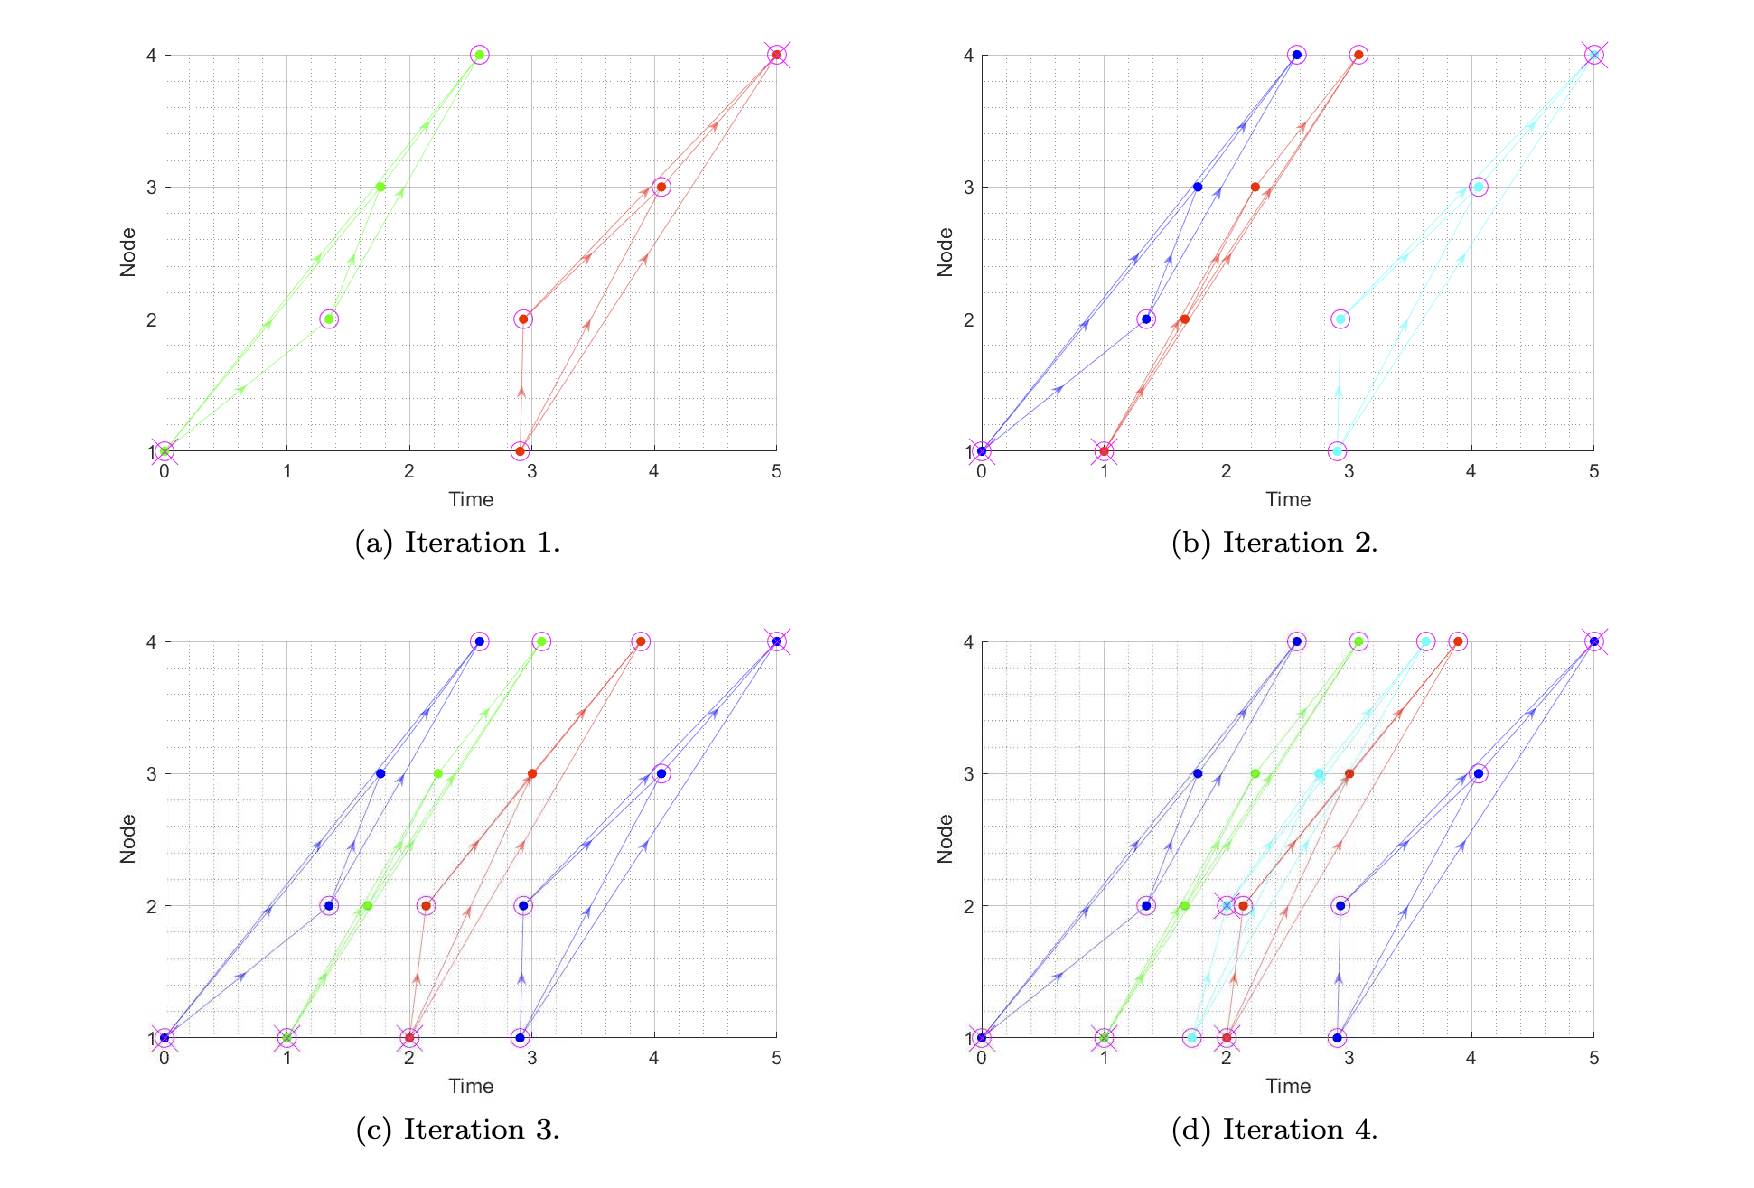
\includegraphics{images/Figure6a.png}
% 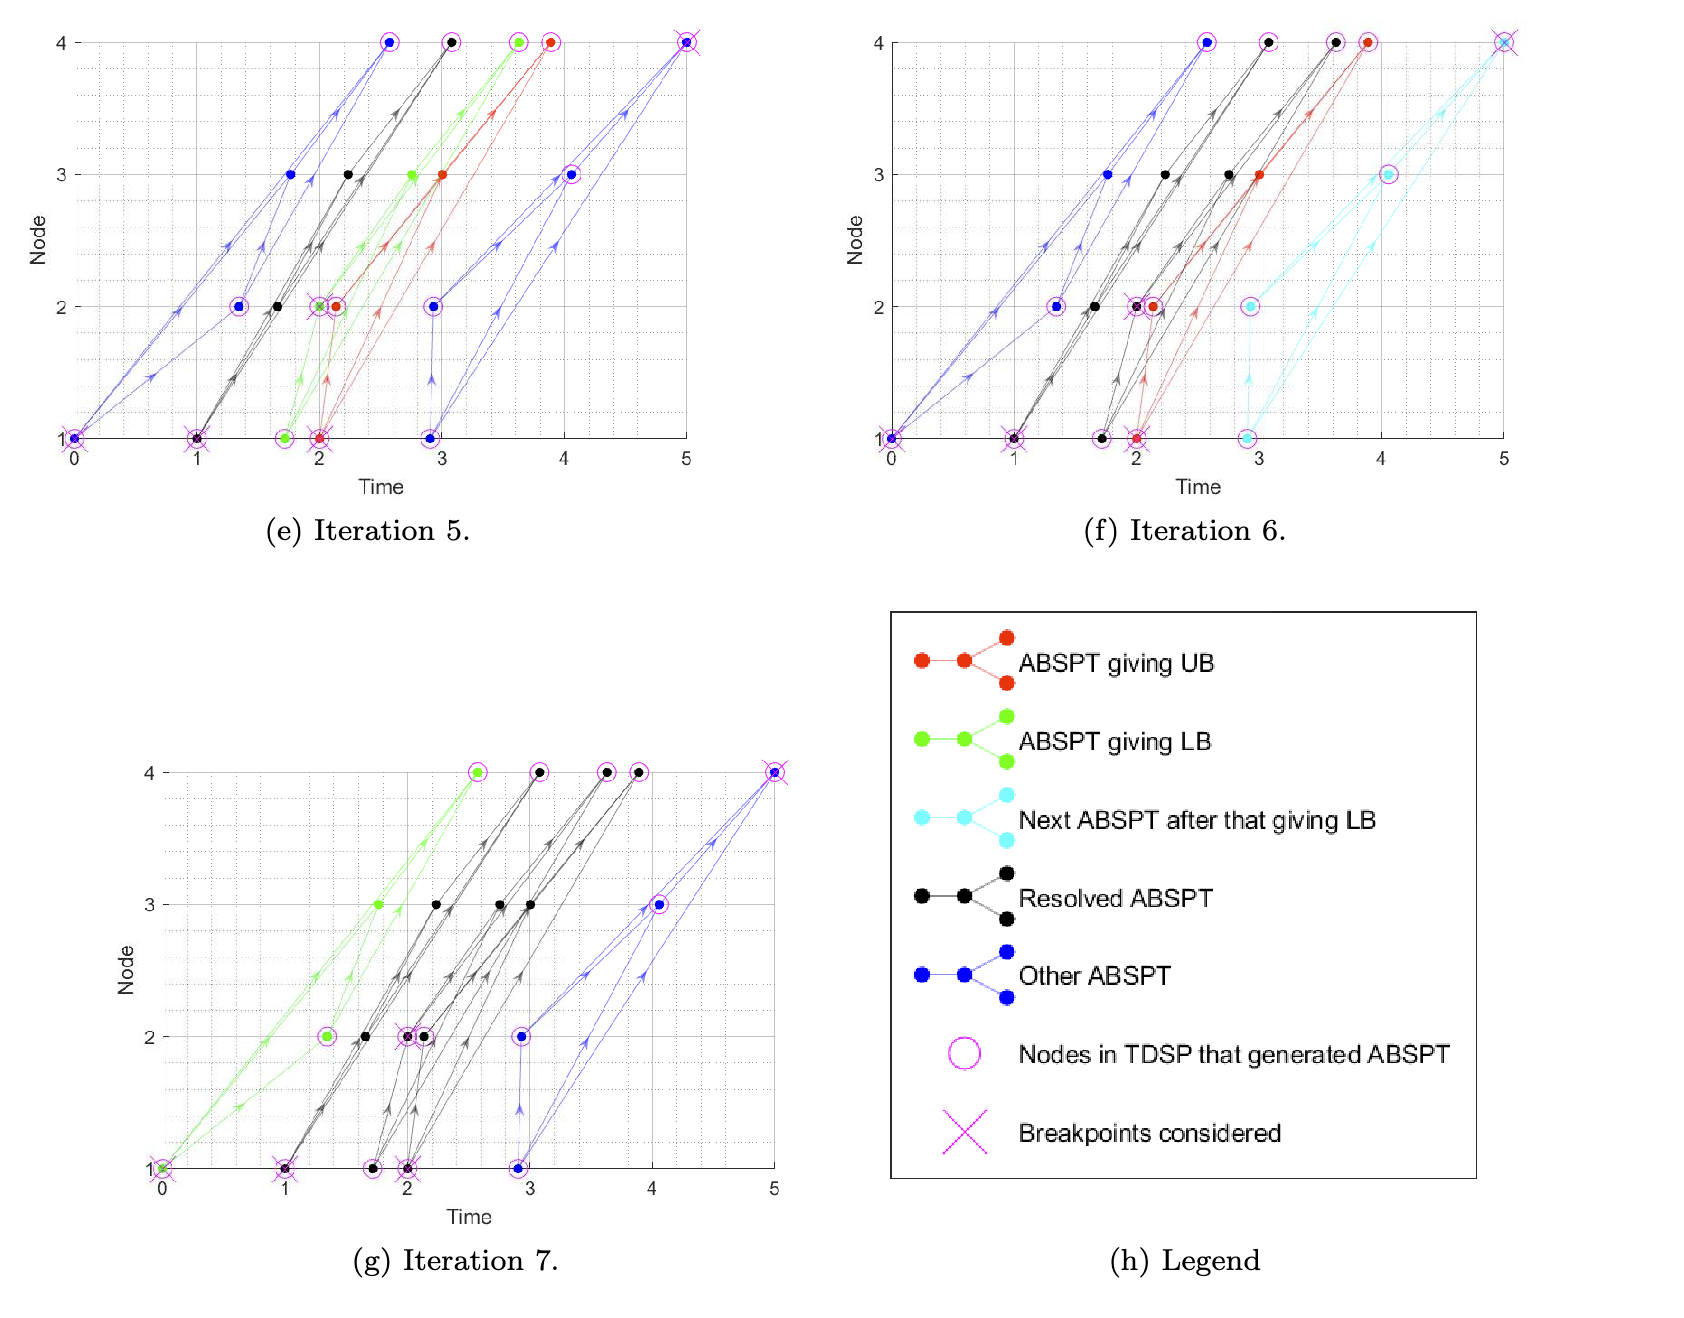
\includegraphics{images/Figure6b.png}
\subcaptionbox{Lần lặp 1\label{fig:6_a}}{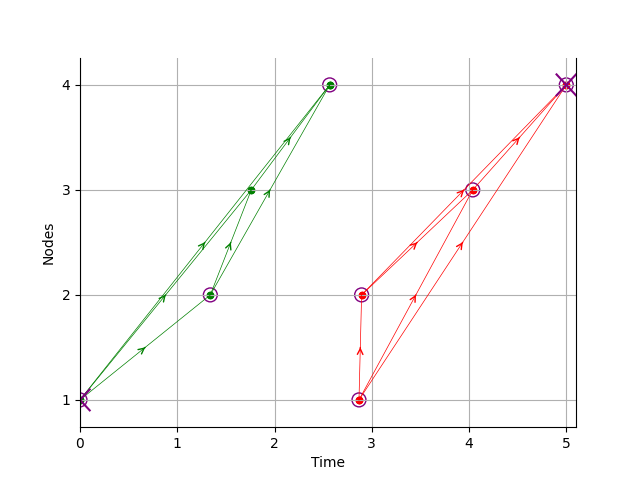
\includegraphics[width=.4\textwidth]{plot2/1 2.png}}
\subcaptionbox{Lần lặp 2\label{fig:6_b}}{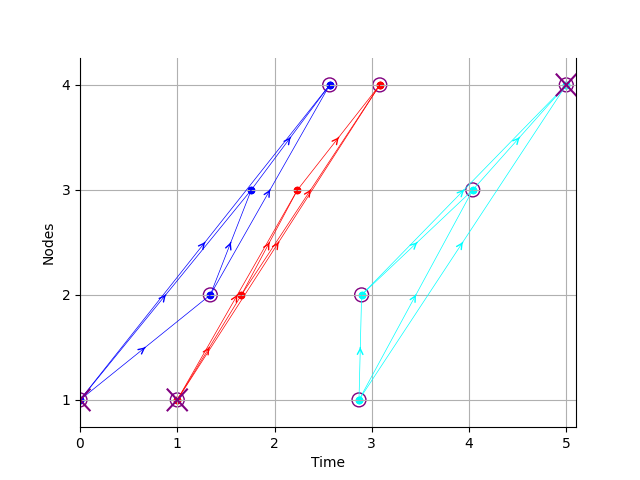
\includegraphics[width=.4\textwidth]{plot2/2 2.png}}
\subcaptionbox{Lần lặp 3\label{fig:6_c}}{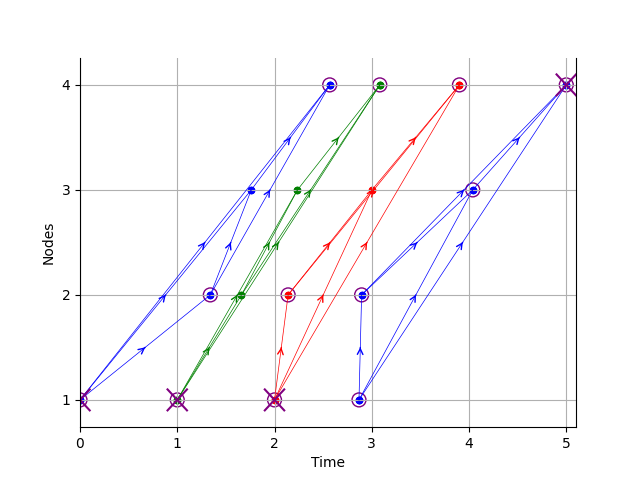
\includegraphics[width=.4\textwidth]{plot2/3 2.png}}
\subcaptionbox{Lần lặp 4\label{fig:6_d}}{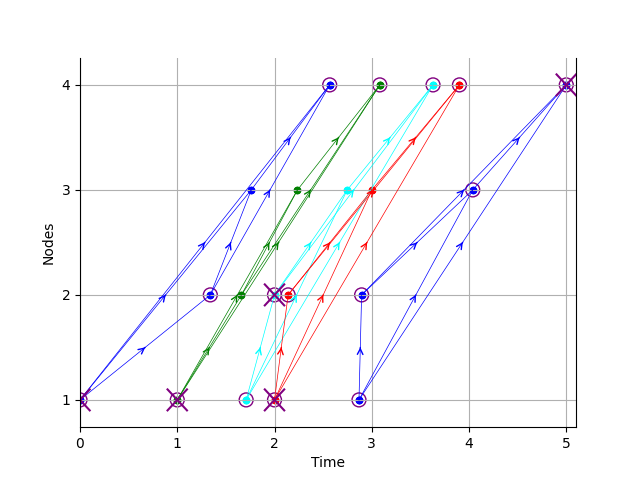
\includegraphics[width=.4\textwidth]{plot2/4 2.png}}
\subcaptionbox{Lần lặp 5\label{fig:6_e}}{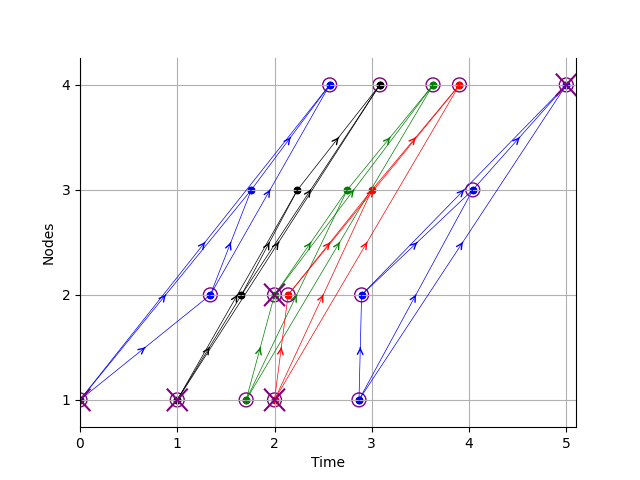
\includegraphics[width=.4\textwidth]{plot2/5 2.png}}
\subcaptionbox{Lần lặp 6\label{fig:6_f}}{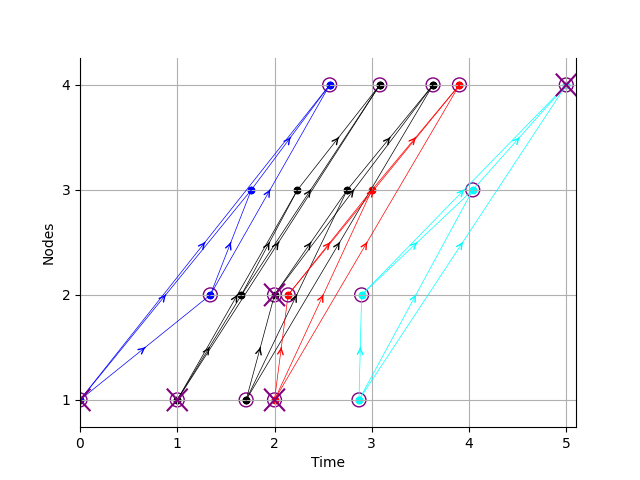
\includegraphics[width=.4\textwidth]{plot2/6 2.png}}
\subcaptionbox{Lần lặp 7\label{fig:6_g}}{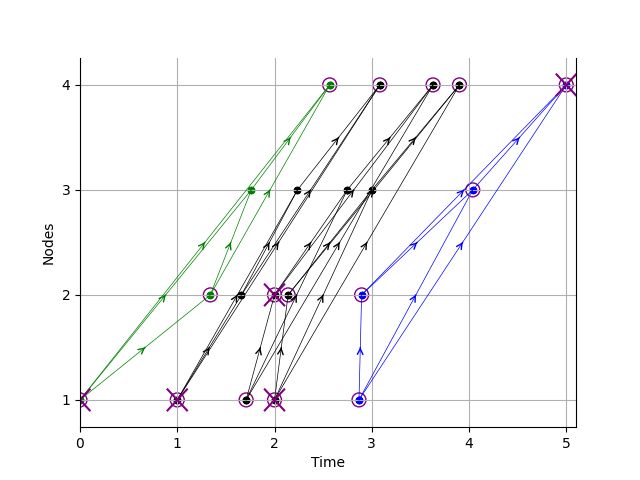
\includegraphics[width=.4\textwidth]{plot2/7 2.png}}
\subcaptionbox{Chú thích\label{fig:6_h}}{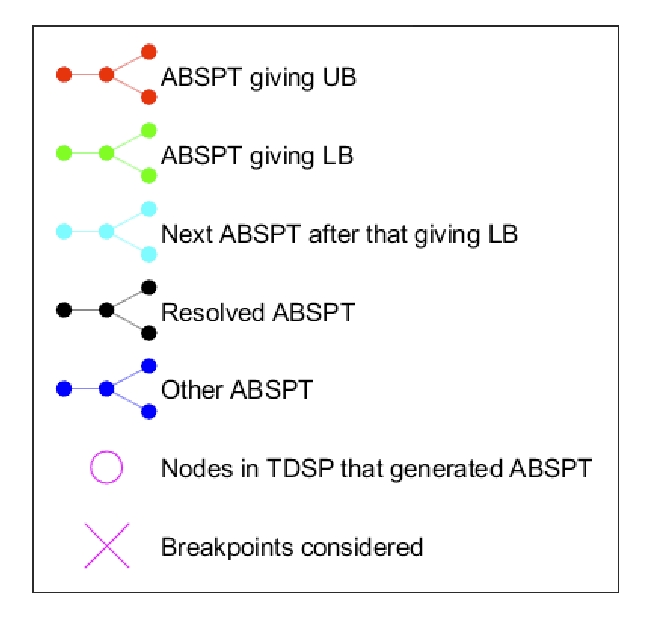
\includegraphics[width=.4\textwidth]{edited-images/Figure6h.jpg}}

\caption{Minh họa cách thức hoạt động của thuật toán trên ví dụ
từ \autoref{fig:2} và \autoref{table:1}.}
\label{fig:6}
\end{figure}


\textbf{Khởi tạo:} Danh sách ABSPT được khởi tạo với hai phần tử:

\begin{itemize}
\tightlist
\item
  \(\overline{\mathcal B}^{2.57}\): ứng với nút \((1, 0)\) - TDSP bắt đầu từ
  \((1, 0)\) đến đỉnh \(4\) tại thời điểm \(t_0 = 2.57\).
\item
  \(\overline{\mathcal B}^{5}\): như đã đề cập ở trên.
\end{itemize}

Các giá trị \(LB=1.25\) và \(UB=2.10\) đã được tính toán ở trên.

\textbf{Lần lặp 1:}

\begin{enumerate}
\def\labelenumi{\arabic{enumi}.}
\tightlist
\item
  Xác định BP \(\tau = 1 \in [0, 2.90]\) của cung \((1, 2)\).
\item
  Tìm thấy BP mới \((j, \tau) = (1, 1)\) giữa hai \textbf{ABSPT}.
\item
  Tìm thấy TDSP \(((1, 1), (2, 1.66), (4, 3.0826))\), đi đến đỉnh \(4\)
  tại thời gian \(3.08\) nên tạo ra \(\overline{\mathcal B}^{3.08}\) và thêm
  vào danh sách (\autoref{fig:6_b}, có 3 ABSPT).
\item
  Cập nhật cận trên và cận dưới: \(UB^{3.08} = 2.08\) và
  \(LB^{3.08} = 1.4\).
\item
  Tính lại và cập nhật cận dưới cho
  \(\overline{\mathcal B}^{2.57} : LB^{2.57} = 1.89.\)
\end{enumerate}

Hiện tại thì \(LB=1.4\) và \(UB = 2.08\). Vì \(LB<UB\) nên tiếp tục
lặp.

\textbf{Các lần lặp tiếp theo:}

\begin{enumerate}
\def\labelenumi{\arabic{enumi}.}
\tightlist
\item
  Thêm ABSPT \(\overline{\mathcal B}^{3.89}\) và
  \(\overline{\mathcal B}^{3.63}\) tương ứng với \((1, 2)\) và \((2, 2)\).
  Cái thứ hai cũng là ABSPT thứ ba trong danh sách tại Lặp 4.
\item
  Cập nhật cận dưới hiện tại: \(LB = 1.71\) (từ
  \(\overline{\mathcal B}^{3.08}\)).
\item
  Do không có BP giữa \textbf{ABSPT} thứ \(2\) và thứ \(3\), cập
  nhật cận dưới của \(\overline{\mathcal B}^{3.08}\) bằng cận trên:
  \(LB^{3.08} \gets 2.08\).
\item
  Cập nhật cận dưới hiện tại: \(LB = 1.89\) (từ
  \(\overline{\mathcal B}^{3.63}\)). (Lặp 5)
\item
  Cập nhật cận dưới của \(\overline{\mathcal B}^{3.63}\) và
  \(\overline{\mathcal B}^{3.89}\) do không còn BP.
\item
  Kiểm tra: \(UB = LB = 1.90\). Thuật toán dừng.
\end{enumerate}

Kết quả nghiệm tối ưu (đường đi tối ưu):
\[((1, 2.00), (2, 2.14), (4, 3.89))\]
\backmatter
\end{document}
% END DOCUMENT